% CVPR 2023 Paper Template
% based on the CVPR template provided by Ming-Ming Cheng (https://github.com/MCG-NKU/CVPR_Template)
% modified and extended by Stefan Roth (stefan.roth@NOSPAMtu-darmstadt.de)

\documentclass[10pt,twocolumn,letterpaper]{article}

%%%%%%%%% PAPER TYPE  - PLEASE UPDATE FOR FINAL VERSION
%\usepackage[review]{cvpr}      % To produce the REVIEW version
\usepackage{cvpr}              % To produce the CAMERA-READY version
%\usepackage[pagenumbers]{cvpr} % To force page numbers, e.g. for an arXiv version

% Include other packages here, before hyperref.
\usepackage{graphicx}
\usepackage{amsmath}
\usepackage{amssymb}
\usepackage{booktabs}
\usepackage{listings}
% It is strongly recommended to use hyperref, especially for the review version.
% hyperref with option pagebackref eases the reviewers' job.
% Please disable hyperref *only* if you encounter grave issues, e.g. with the
% file validation for the camera-ready version.
%
% If you comment hyperref and then uncomment it, you should delete
% ReviewTempalte.aux before re-running LaTeX.
% (Or just hit 'q' on the first LaTeX run, let it finish, and you
%  should be clear).
\usepackage[pagebackref,breaklinks,colorlinks]{hyperref}


% Support for easy cross-referencing
\usepackage[capitalize]{cleveref}
\crefname{section}{Sec.}{Secs.}
\Crefname{section}{Section}{Sections}
\Crefname{table}{Table}{Tables}
\crefname{table}{Tab.}{Tabs.}
\lstset{
	basicstyle=\fontsize{8}{10}\selectfont\ttfamily
}
\graphicspath{{images}}

%%%%%%%%% PAPER ID  - PLEASE UPDATE
\def\cvprPaperID{*****} % *** Enter the CVPR Paper ID here
\def\confName{CVPR}
\def\confYear{2023}


\begin{document}

%%%%%%%%% TITLE - PLEASE UPDATE
\title{Deep Learning Fundamentals\\
	Assignment 2 - Butterfly classification: Using CNN models}

\author{Zeyu Zuo\\
The University of Adelaide\\
{\tt\small a1894365@adelaide.edu.au}}
\maketitle

%%%%%%%%% ABSTRACT
\begin{abstract}
The conventional method for identifying butterfly species such as the examination of colour, 
shape and patterns of wings or dissection of butterflies. These approached can be 
time-consuming, expensive and potentially harmful to the specimens. 
This paper aims to improve
the effectiveness of butterfly classification by find the suitable pretrained architecture among Resnet34, Reset 50, Vgg16, Vgg19, Efficientnetb0, Efficientnetb2, Vit
,instantly identify the butterfly species from images with high accuracy. 
the results of all the proposed models were compared and evaluated using accuracy,Precision ,Recall and F1Score. 
The results of the investigation indicates that VisionTransfomer architecture outperforms all other archiitectures, achieving an accuracy rate of 95.08%.
\end{abstract}

%%%%%%%%% BODY TEXT
\section{Introduction}
\label{sec:intro}

Butterflies is a category of insects within the Lepidoptera family with approximately 28000 species distributed widely across the world's ecosystems\cite{ghazanfar2016butterflies} . They not only contribute to the Earth's biodiversity and serve as indicators of environmental conditions and changes, but they also offer a multitude of ecosystem services and direct advantages to humans such as pollinate plants and applicate in dyes, medicines and researches \cite{wang2020butterfly}. \\
\indent The traditional method of butterfly identification is capturing desired butterfly species and observing various morphological characteristics, including size, wing venation, colour, shape, and patterns. Some visually similar butterflies require in-depth studies, including dissection and molecular techniques, making the identification process laborious and time-consuming while potentially harming the insects due to the longtime confinement \cite{xi2022multiple}.To address these problems, there is a growing need for the development of intelligent digital systems capable of straightforward and accurately categorise butterflies using images.
\\
\indent The development of advanced progress in artificial intelligence systems has provided effective solutions in tasks related to the classification of images.The technique commonly
Applied to image detection, segmentation and recognition is the Convolution Neural Network(CNN), which known for its efficiency in extracting meaningful features from raw data,reduces 
the need for extensive data preprocessing and enhances their adaptability to a variety of tasks. The most popular pre-trained CNN available are ResNet, ViT, GoogLeNet, EfficientNet and inception. 

\indent The aim of this paper is to analyse pre-trained machine learning models with the implementation of CNN to find a one that can effectively categorise butterfly images with high accuracy and low loss on training and validation data. The dataset including data augmentation to prevent overfitting and underwriting along with applying the technique of transfer learning to improve generalisation and speed up training. To attain the highest level of accuracy and evaluate each model, a performance assessment conducted using accuracy, precision, recall, and F1 score as evaluation metrics.

\section{Related work}
To identify butterflies, early researchers used texture\cite{kaya2015automatic}, color features \cite{kaya2015automatic}, Branch Length Similarity (BLS) entropy{kang2012butterfly}, and wing shape outlines\cite{kang2014identification}. Some of the early butterfly research used feature extraction techniques, such as the gray-level co-occurrence matrix (GLCM) and local binary patterns (LBP) in butterfly feature spaces, to classify 190 butterfly images belonging to 19 different species of the Pieridae family with an accuracy of 98.25\% and 96.45\% \cite{kaya2014evaluation}.\\

\indent However, in recent years, due to advancements in artificial intelligence algorithms and graphical processing units (GPUs), convolutional neural networks (CNN) have been applied to image classification. The advantages lies in their ability to automatically extract relevant features from the dataset, solving fine-grained complex classification problems, and achieving the expected results. 

Silva et al.\cite{rashid2020sustainable} 
aimed to determine the best feature selection strategies and classifiers for identifying honeybee subspecies among seven feature pickers and classification methods. In their experiments, they discovered that the best combination was the naive Bayes classifier and mutual information feature extraction.

Hernandez et al.\cite{hernandez2014automatic} 
used computational methods to categorize 740 species and 11,198 samples in a dataset. They achieved an accuracy of 91.65\% for fish, 92.87\% for flora, and 91.25\% for butterflies.
\\
\indent 
Wen et al.\cite{hernandez2014automatic} 
incorporated both local and global information for insect classification. They developed a model that combines various classification methods, including K nearest neighbor classification (KNNC), regular densities predicted sequential classification model (NDLC), minimal level fewest linear classification algorithm (MLSLC), the nearest mean classifier (NMC), and decision tree (DT). Their experimental results showed an 86.6\% classification rate when assessed on images taken during actual field trapping for training.\\
\indent 
Xie et al.\cite{xie2018automatic} 
created a butterfly dataset that includes both standard pattern images and images from the natural environment. The dataset consisted of 5695 images representing all 1176 butterfly species from China. The dataset was trained using Faster-RCNN and achieved a mean average precision (mAP) of 60\%.\\
\indent 
Zhu et al.\cite{zhu2019towards}proposed a comprehensive approach that combines region matching and the dual-complex discrete wavelet method for classifying lepidopteran insect images. They tested their method on a collection of 100+ lepidopterous insects from 18 genera and achieved a recognition accuracy of 84.47\%.\\
\indent 
Nur Nabila Kamaron Arzar et al.\cite{arzar2019butterfly} have proposed the use of the GoogleNet pre-trained model to classify butterfly images. The study involved a dataset of 120 butterflies categorised into four distinct classes with the result of 90.5\% overall identification accuracy. However, this sample size was relatively small, leading to overfitting and inaccurate recognition on new data.\\
\indent 
These studies reflect the evolution of techniques and methods in butterfly classification, from traditional feature extraction to the application of deep learning and advanced algorithms.
\section{Methodology}
\label{sec:related}

\subsection{Dataset Description}{Dataset description } The dataset contains more than 1000 images of 75 species butterflies from around the world. The dataset has been divided into two parts: 80
\% for training data and 20\% for validation. The images were sourced from Kaggle and were resized to a uniform resolution of 240x240 pixels, as they originally had varying resolutions.

\subsection{Data augmentation} Data augmentation is a widely used technique in deep learning to artificially increase the size of training dataset by applying various transformations to the existing data. Implementation data augmentation enable the generation of additional images improving the robustness and generalisation of the model to effectively handle diverse scenarios, including irregularities in the shape, texture, and colour of butterflies\cite{o2020deep}.\\
\subsubsection{Transform}

\textbf{HorizontalFlip and VerticalFlip:} Flips the image to create a mirrored version, helping the model recognize objects oriented left to right and upside down.

\textbf{RandomBrightnessContrast:} This processing randomly adjusts the image's brightness and contrast to help the model adapt to different lighting conditions.

\textbf{HueSaturationValue:} This technique randomly modifies the hue, saturation, and value of the image to improve the model's ability to handle variations in color and color intensity.

\textbf{CoarseDropout:} Introduces random, block-like patches of missing data in the images to help the model focus on the relevant features.

\subsection{Batch Normalisation} Batch normalisation was proposed by Sergey Ioffe and Christian Szegedy in 2015 and described using the following formula:

\begin{equation}
    \hat{x} = \frac{x - \mu}{\sqrt{{\sigma}^2 + \epsilon}} \cdot \gamma + \beta
\end{equation}

where $x$ is the input to the BatchNorm layer, $\mu$ is the mean of the mini-batch, $\sigma^2$ is the variance of the mini-batch, $\gamma$ is the scale parameter, $\beta$ is the shift parameter, and $\epsilon$ is a small constant.\\
\indent The purpose is to normalize the input feature distribution (subtracting mean and dividing by standard deviation) to every training mini-batch, allowing the model improve gradient flow through the network and reduce the strong independence on initialisation\cite{ioffe2015batch}.

\subsection{Convolutional Neural Network} The CNN was developed from the Multilayer Perceptron (MLP), a network primarily designed for processing two-dimensional data. The basic structure of a CNN consists of an input layer, convolutional layers, pooling layers, fully connected layers, and an output layer. In the convolutional layers, each neutron in the output feature map is locally connected to its input. It computes a weighted sum of the local inputs using corresponding connection weights and adds a bias value to obtain the input value for that neutron\cite{lecun2015deep}. A CNN image shows in Figure 1.

\begin{figure}[t]
	\centering
	\includegraphics[width=\columnwidth]{butterfly}
	\caption{Right is a predicted butterfly classic , left is imput image.}
	\label{fig:svm-lr}
\end{figure}


\subsubsection{ Convolution layer} 
The aim of convolution layer is to extract different features from input data by computing the dot product between the regions of the input image and the weight matrix of the filter, and this result becomes the output of that layer\cite{krizhevsky2012imagenet}. The convolution layer is calculated as follow:
\begin{equation}
    \hat{F}_{j} = \sum_{i} F_{i} \otimes K_{i,j} + b_{j}
\end{equation}


$\hat{F}_{j}$ represents the output feature map or activation map for the $j$-th feature map in the convolutional layer. 
$F_{i}$ corresponds to the $i$-th input feature map from the previous layer or the input data.
$\otimes$ denotes the 2D convolution operation, which is a mathematical operation that combines the input feature map $F_{i}$ with the kernel $K_{i,j}$ to compute the output feature map $\hat{F}_{j}$. 
$K_{i,j}$ is the kernel (also known as a filter) used for the convolution operation. 
$b_{j}$ represents the bias term associated with the $j$-th output feature map. It's added to the result of the convolution operation to introduce an offset or shift in the output.

\subsubsection{ Pooling layer} 
The function of pooling layer is to reduce the dimensions of the feature maps through down-sampling and minimise the parameters, spending up the computation time without reducing depth. In this task ,the dimension of feature maps is reduced by performing max-pooling operation,the pooling layer sliding the filter over the output feature map of the previous convolution layer and keeps the maximum value of each grid\cite{scherer2010evaluation}.
\begin{equation}
    f_M(X) = \max_{i,j}(i,j)
\end{equation}

$X$ represents the input matrix or grid.
$i$ and $j$ represent the indices of the elements within the grid. The max pooling operation is applied by sliding a typically $2 \times 2$ or $3 \times 3$)kernel over the input grid $X$ to perform the pooling operation at each position $(i, j)$.

\subsubsection{ Fully connected layer} 
The purpose of fully connected layer is to flatten the output of the previous layer by applying a linear transformation to the input vector through a weights matrix because the subsequent dense layers can only receive 1D vectors.The output is fixed as the number of classed used. 

\subsection{Transfer learning }

Transfer learning is the practice of applying knowledge acquired from one task to enhance the performance in a related task\cite{chang2017fine}. In this context, a butterfly image classification (target task) can be learned by leveraging the generic features learned from the natural image classification (source task) .The model remove the original fully connected layers, and use the learning rate to fine-tune the entire network weights. Transfer learning facilitates the recycling and transference of acquired knowledge on related domains and reduce the cost of model training.

\subsection{ Architecture }
\subsubsection{ResNet} 
ResNet, short for Residual Network, was introduced by Kaiming He and his colleagues in 2015\cite{he2016deep}. The fundamental idea behind it is to skip convolutional layer blocks using shortcut connections. These basic blocks are referred to as "bottleneck" blocks and apply residual connections between convolutional layers, followed by passing through ReLU activation layers. Residual connections ensure that weights learned from earlier layers do not vanish during backpropagation. ResNet-34 consists of 34 convolutional layers and has approximately 218,000 parameters. ResNet-50, on the other hand, is deeper with 50 convolutional layers and typically has around 256,000 parameters.
The schematic representation of ResNet50 model is shown in Fig 2.
\begin{figure}[h]
    \centering
    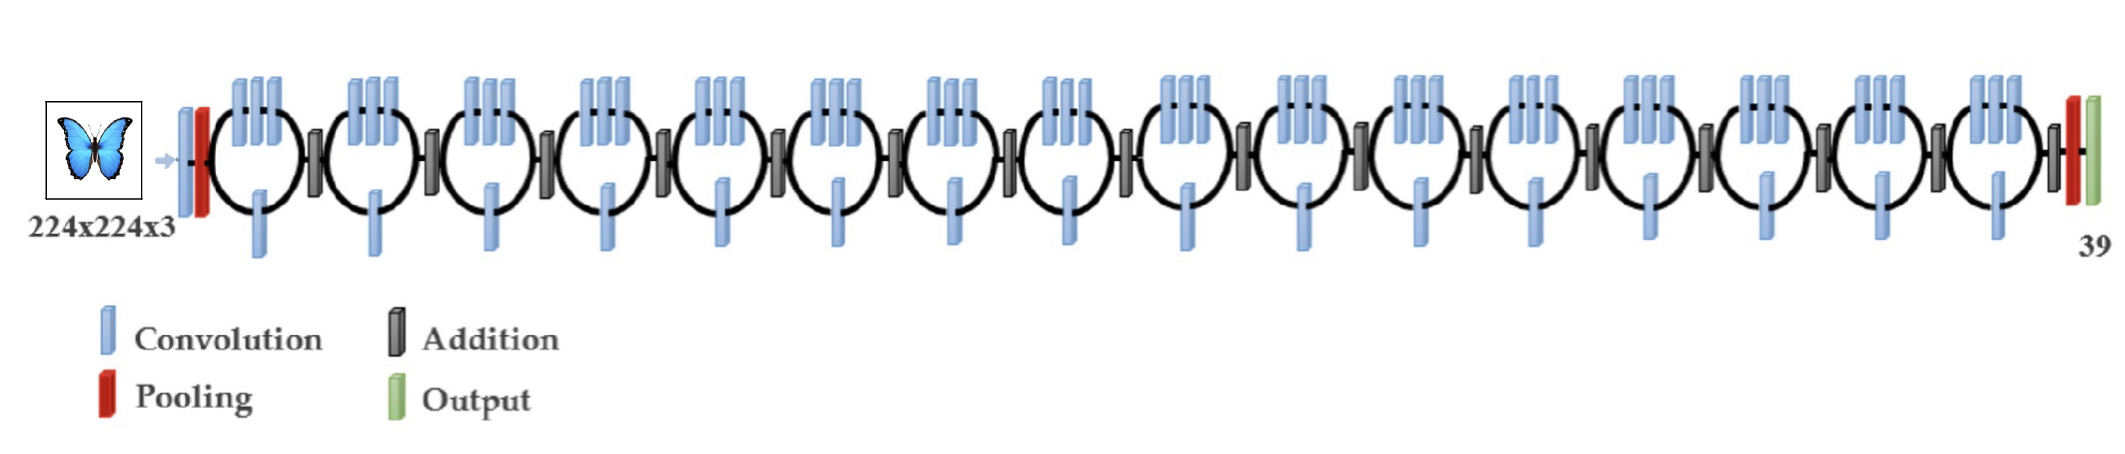
\includegraphics[width=\columnwidth, height=1.1in]{res50} % Adjust the height value as needed
    \caption{}
    \label{fig:svm-lr}
\end{figure}



\subsubsection{ VGG Network Architecture}

VGG16 and VGG19 were proposed by Simonyan and Zisserman from the Visual Geometry Group at the University of Oxford in 2014\cite{simonyan2014very}.

The VGG16 architecture consists of 138,355,752 parameters and includes 
five convolutional blocks and three fully connected layers ,
 the first two utilising ReLU activation, and the final one employing the Softmax activation 
 function. Each block comprises several convolutional layers followed by a max-pooling 
 layer, which serves to reduce the block's output size and eliminate noise.
 The different between VGG and other architecture is that VGG has a relatively small number of hyper-parameters and total 16 layers. 
 it has the same convolution layers with stride 1 and same padding and maximum pooling layers. 
 This consistent pattern of convolution and pooling layers is maintained throughout the entire architecture.
 The input layer of this architecture accepts images with dimensions of 224x224 pixels.The schematic representation of VGG16 model is shown in Fig 3.
\begin{figure}[h]
	\centering
	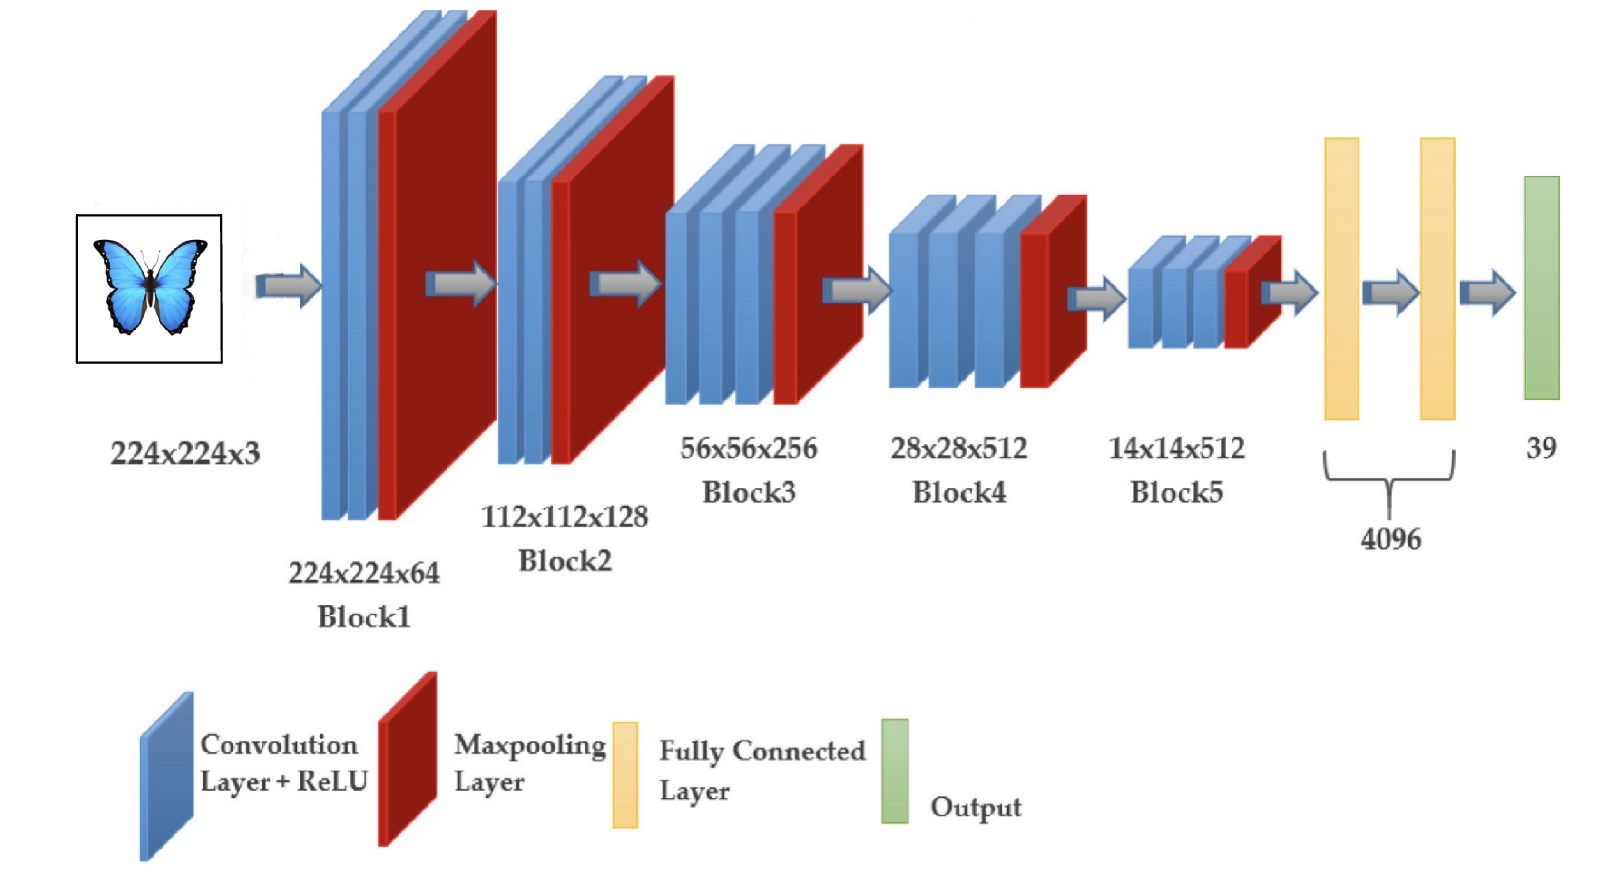
\includegraphics[width=\columnwidth]{vgg16}
	\caption{}
	\label{fig:svm-lr}
\end{figure}

 For VGG19 , it contains 19 convolutional layers, resulting in 143,667,240 parameters due to the inclusion of additional layers. Pre-trained VGG16 and VGG19 models, trained on extensive datasets like ImageNet, can be employed as a starting point for transfer learning , saving time and resources compared to training from scratch.

\subsubsection{EfficientNet} 
EfficientNet, a state-of-the-art image classification model, has achieved an impressive 84.4\% accuracy on the ImageNet classification task with parameter count of 84 million. It accomplishes its efficiency by uniformly adjusting the dimensions of depth, width, and resolution. The initial phase of their scaling method involves a grid search to establish the interplay between scaling dimensions while adhering to resource constraints. This process identifies suitable scaling factors for depth, width, and resolution, which are then applied to scale the baseline network to the desired target model. In contrast to other convolutional neural network models, EfficientNet adopts a novel activation function known as Swish, in contrast to the commonly used Rectified Linear Unit (ReLU). The EfficientNet family consists of eight models, labeled from b0 to b7. In the context of a butterfly classification model, this paper specifically compared the pre-trained EfficientNet B0 and B2 models. A visual representation of the EfficientNet B0 model is provided in Figure 4.
\begin{figure}[t]
	\centering
	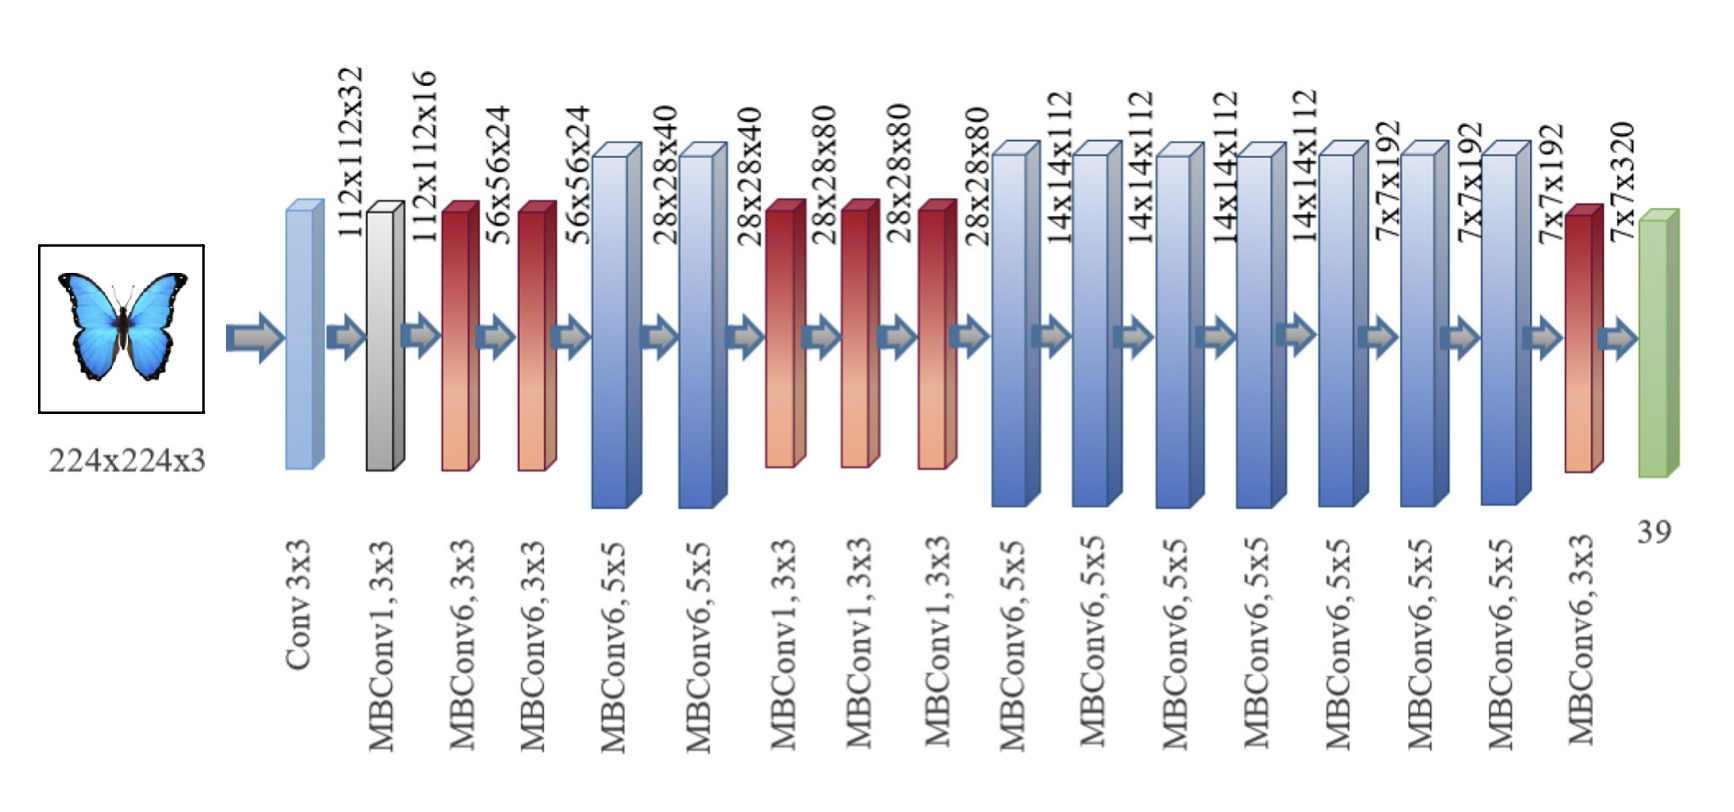
\includegraphics[width=\columnwidth]{effb0}
	\caption{}
	\label{fig:svm-lr}
\end{figure}


\subsubsection{VisionTransfomer} 
ViT is a model that applies the Transformer architecture to image classification. ViT works by dividing the input image into multiple patches, then projecting each patch into a fixed-length vector, which is subsequently processed using self-attention mechanisms\cite{wu2021vision}. The operations in the following encoder are identical to the original Transformer. A special token is added to the input for image classification. The output corresponding to this token represents the final class prediction.The difference between traditional CNN architectures, which typically utilize filters with limited local receptive fields, and the Vision Transformer is that Vit has attention mechanism enables it to focus on various regions of the image and effectively incorporate information from across the entire image\cite{bazi2021vision}.

\subsection{Optimizer}
During network training, the primary task of the optimizer is to update the model's weights in order to minimize the loss function. This enables the model to discover the optimal combination of parameters and learn from the provided training data. The choice of optimizer can significantly impact the convergence of the training process, particularly in the context of transfer learning.\\

\indent The Adam algorithm utilizes the Hessian matrix, includes second-order derivatives. The advantages is reducing memory usage and the need for fewer computational resources\cite{kingma2014adam}. Adam operates by calculating an adaptive learning rate for each parameter in the model, combining the strengths of both Momentum and RMSprop and adjusts the learning rate using squared gradients\cite{zhang2018improved}.


\subsection{ Loss function} 
The model employ categorical cross-entropy as loss function. The loss function is defined as follows:

\begin{equation}
    \mathcal{L}(y,\hat{y}) = -\frac{1}{M}\sum_{j=0}^{M}\sum_{i=0}^{N}(y_{ij} \ast \log(\hat{y}_{ij}))
\end{equation}
Where:
$\hat{y}$ represents the predicted probability.
$y$ is the actual probability.
$M$ is the number of mini-batch.
$N$ represents the number of butterfly species in the dataset.


\section{ Experiment} 
\subsection{Tools} 
The framework uses PyTorch\cite{paszke2019pytorch}and FastAi\cite{howard2020fastai} framework. Data augmentation techniques applied using Albumentations. The hardware configuration includes an Apple Silicon M2 with 32GB of RAM and an NVIDIA Tesla P4 with 8GB of VRAM, along with an Intel 6-core processor and 64GB of RAM. All models are trained and fine-tuned using 32-bit floating-point precision.

\subsection{Metrics} 
The performance of butterfly classifier efficiency was evaluate based on Accuracy, Precision, Recall and F1score. Accuracy is a straightforward metric that measures the proportion of correctly classified instances among all instances in the dataset. where TP identifies the True Positive, TN identifies the True Negative, FP identifies the False Positive and FN identifies the False Negative.

\begin{equation}
	Accuracy = \frac{TP+TN}{TP+TN+FP+FN}
\end{equation}
\indent Precision represents the probability that a sample predicted as positive is actually positive. Precision measures the accuracy of positive predictions, while accuracy considers both positive and negative predictions.
\begin{equation}
	Precision = \frac{TP}{TP+FP}
\end{equation}

\indent  Recall calculates the proportion of true positive predictions among all actual instances of the class.Higher recall indicates a higher probability of correctly identifying actual positive cases.
\begin{equation}
	Recall = \frac{TP}{TP+FN}
\end{equation}
\indent The F1 Score is the harmonic mean of precision and recall. It provides a balanced measure of a model's performance, especially when precision and recall are in conflict.
\begin{equation}
	F1-Score = \frac{2\times Precision\times Recall}{Precision+Recall}
\end{equation}




\subsection{Result} 
In this experiment, I conducted butterfly classification using various pre-trained models. The models were trained for 20 epochs with a batch size of 32.
The table below showcases the evaluation results of different pre-trained models. \\

\begin{table}[h]
    \small
    \setlength{\tabcolsep}{3.5pt}
    \begin{tabular}{@{}lccccccc@{}}
        \toprule
        & PARAMs & Loss & Accuracy & Precision & Recall & F1Score \\
        \midrule
        vgg16 & 138 & 0.4552 & 0.8669 & 0.8732 & 0.8710 & 0.8678 \\
        vgg19 & \color{red}\textbf{144} & 0.47049 & 0.8661 & 0.8704 & 0.8740 & 0.8681\\
        effNet\_b0 & \color{green}\textbf{5.3} & 0.3083 & 0.9215 & 0.9278 & 0.9251 & 0.9247 \\
        effNet\_b2 & 9.2 & 0.3008 & 0.9185 & 0.9227 & 0.9199 & 0.9190 \\
        resnet34 & 21.5 & 0.4284 & 0.8862 & 0.8901 & 0.8897 & 0.8869 \\
        resnet50 & 23.9 & 0.3127 & 0.9292 & 0.9340 & 0.9311 & 0.9309 \\
        vit\_base & 86 & \textbf{0.2913} & \textbf{0.9508} & \textbf{0.9533} & \textbf{0.9553} & \textbf{0.9528} \\
        \bottomrule
    \end{tabular}
\end{table}

\textbf{Note}: PARAMs represent the number of parameters in millions.\\


Notably, the Vision Transformer (VIT) with a base configuration outperforms other models in terms of both accuracy and F1 score.It achieved an impressive accuracy of 95.08\%.The high precision, recall, and F1 score further highlight the VIT's capability to accurately classify butterfly species.Meanwhile, EfficientNet also achieved relatively ideal results, with an accuracy of around 92\%. In particular, EfficientNet B0, with the fewest parameters among other models at only 5.2 million, performed even slightly better than EfficientNet B2. ResNet architectures are known for their depth, which can sometimes lead to vanishing gradient problems during training. This issue becomes more pronounced in this particular task due to the relatively small dataset of just over 1000 butterfly images. Consequently, these challenges can lead to slower convergence and reduced accuracy. VGGnet has the highest number of parameters among the models used, and its training time is the longest, but the training results are not ideal. In summary, EfficientNet B0 and Vision Transformer Base are better suited for butterfly classification in this task due to their efficient parameter usage and superior performance on the given metrics.


\section{Conclusion} 
The paper compares common and effective pre-trained transfer-learning models for identifying specific butterfly species by analyzing butterfly visual images. Due to the limited number of butterfly images collected by Kaggle, data augmentation techniques were employed to acquire more images.The proposal leverages transfer-learning algorithms to facilitate the efficient identification of butterfly species, utilizing pre-trained transfer-learning neural network models such as VGG16, VGG19, Efficientnetb0, Efficientnetb2, Resnet34, ResNet50, and Vision Transformer.These models classified 75 different butterfly species in total, and their performances were validated using a validation dataset, all of them exhibiting the expected efficiency.Performance metrics used to evaluate the models included accuracy, precision, recall, and F1 scores. Among all the models, ViT with data augmentation achieved the highest accuracy, reaching 95.08\%. The butterfly dataset used in the experiments consisted of images from various species, with different quantities for each species. This imbalance in image data could result in bias in the butterfly dataset, leading to generalization errors. Additionally, the number of images for each butterfly species was limited. Therefore, in the future, it would be beneficial to collect and add more images for each species. More multimodal data from real-time videos, including both images and sounds of species, can also be included as input for pre-trained models to improve the accuracy of evaluation results.










	%%%%%%%%% REFERENCES
	{\small
		\bibliographystyle{ieee_fullname}
		\bibliography{egbib}
	}

\end{document}
